\documentclass[a4paper,12pt]{article}
\usepackage{amsmath, amssymb}
\usepackage{geometry}
\usepackage{enumitem}
\usepackage{fancyhdr}
\usepackage{xcolor}
\usepackage{sectsty}
\usepackage{multicol}
\usepackage{graphicx}
\usepackage{float}
\def\inputGnumericTable{}
\usepackage[latin1]{inputenc}
\usepackage{fullpage}
\usepackage{color}
\usepackage{array}
\usepackage{longtable}
\usepackage{calc}
\usepackage{multirow}
\usepackage{hhline}
\usepackage{ifthen}
\geometry{top=1in, bottom=1.5cm, left=1.5cm, right=1.5cm}    % Header and Footer settings
\pagestyle{empty}
\sectionfont{\color{blue}}
\begin{document}

\thispagestyle{fancy}
\fancyhf{} % Clear default header and footer
\fancyhead[L]{% Left header
        
\includegraphics[width=8cm, height=1.7cm]{images/logo.png} % Adjust dimensions
}
\fancyhead[R]{% Right header
    Name: M.Thrinath Rao \\
    Batch: COMETFWC034 \\
    Date: 05 September 2025
}
\renewcommand{\headrulewidth}{0pt} % Remove header line
\fancyfoot[C]{\thepage} % Page number centered in footer
\vspace*{1cm}
\begin{center}
        {\LARGE \textbf{\textcolor{blue}{GATE 2010 EC, $39^{th}$ Question Analysis}}}
\end{center}
\section*{\textbf{Question 39}}
The Boolean function reaized by the logic circuit shown is
\begin{center}
        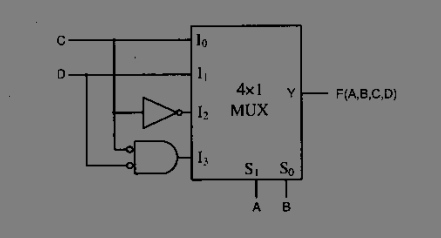
\includegraphics[width=12cm, height=8cm]{images/circuit.jpg}
\end{center}
\begin{multicols}{2}
                \begin{enumerate}[label=\Alph*]
			\item $F = \sum m(0,1,3,5,9,10,14)$
			\item $F = \sum m(2,3,5,7,8,9,12,13)$
			\item $F = \sum m(1,2,4,5,11,14,15)$
			\item $F = \sum m(2,3,5,7,8,9,12)$
                \end{enumerate}
\end{multicols}
\section*{\textbf{Question Analysis:}}
\begin{itemize}
        \item The standard mux equation of 4x1 mux is
	\item $F = \bar{S_{1}}.\bar{S_{0}}.I_{0} + \bar{S_{1}}.S_{0}.I_{1} + S_{1}.\bar{S_{0}}.I_{2} + S_{1}.S_{0}.I_{3}$
	\item here $S_{1}=A, S_{0}=B, I_{0}=C, I_{1}=D, I_{2}=\bar{C}, I_{3}=\bar{C}.\bar{D}. $
	\item So $F = \bar{A}.\bar{B}.C + \bar{A}.B.D + A.\bar{B}.\bar{C} + A.B.\bar{C}.\bar{D} $
	\item The conanical form of $F$ is as follows
	\item $F = \bar{A}.\bar{B}.C.\bar{D} + \bar{A}.\bar{B}.C.D + \bar{A}.B.\bar{C}.D + \bar{A}.B.C.D + A.\bar{B}.\bar{C}.\bar{D} + A.\bar{B}.\bar{C}.D + A.B.\bar{C}.\bar{D}$
        \item The Truth table for above expressions is as follows
	\item From Truth Table we can see that Option-D is correct.
\end{itemize}
\newpage
\section*{\textbf{The Truth Table}}
\begin{center}
\begin{tabular}{|c|c|c|c|c|}
\hline
	\multicolumn{4}{|c|}{\textbf{INPUTS}} & \textbf{Output} \\ 
\hline
	$A$ & $B$ & $C$ & $D$ & $F(A,B,C,D)$ \\
\hline
0 & 0 & 0 & 0 & 0 \\ 
0 & 0 & 0 & 1 & 0 \\ 
0 & 0 & 1 & 0 & 1 \\ 
0 & 0 & 1 & 1 & 1 \\ 
0 & 1 & 0 & 0 & 0 \\ 
0 & 1 & 0 & 1 & 1 \\ 
0 & 1 & 1 & 0 & 0 \\ 
0 & 1 & 1 & 1 & 1 \\ 
1 & 0 & 0 & 0 & 1 \\ 
1 & 0 & 0 & 1 & 1 \\ 
1 & 0 & 1 & 0 & 0 \\ 
1 & 0 & 1 & 1 & 0 \\ 
1 & 1 & 0 & 0 & 1 \\ 
1 & 1 & 0 & 1 & 0 \\ 
1 & 1 & 1 & 0 & 0 \\ 
1 & 1 & 1 & 1 & 0 \\ 
\hline
\end{tabular}
\end{center}
\section*{\textbf{Hardware Implementation}}
The above problem is implemented and tested in hardware using Arduino UNO board. Here we used the 7447 and 7474 and displayed the corresponding F value on LED and respective min term on seven segment as per truth table using FSM and verified the expression.
\section*{Required Components \& Pin Connections}
\begin{center}
\begin{minipage}{0.45\textwidth}
\begin{table}[H]
\centering
\begin{tabular}{|c|l|}
\hline
\textbf{S.No} & \textbf{Component} \\ \hline
1 & Arduino Uno Board \\
2 & Breadboard \\
3 & 7447 IC (1) \\
4 & Seven segment (1) \\
5 & Resistors: 220$\Omega$ (1) \\
6 & Jumper Wires \\
7 & USB Cable \\
8 & 7474 IC (2) \\
9 & LED (1) \\
\hline
\end{tabular}
\end{table}
\end{minipage}
\hspace{0.05\textwidth}
\begin{minipage}{0.45\textwidth}
\begin{table}[H]
\centering
\begin{tabular}{|c|c|}
\hline
\textbf{Component} & \textbf{Arduino Pin} \\ \hline
Input A(GND or 5v) & Digital 5 \\
Input B(GND or 5v) & Digital 4 \\
Input C(GND or 5v) & Digital 3 \\
Input D(GND or 5v) & Digital 2 \\
Output F (LED) & Digital 8 \\
Output a (7474-1 D1) & Digital 9 \\
Output b (7474-1 D2) & Digital 10 \\
Output c (7474-2 D1) & Digital 11 \\
Output d (7474-2 D2) & Digital 12 \\
Output clk (7474 clk) & Digital 13 \\
GND & GND \\
VCC & 5V \\
\hline
\end{tabular}
\end{table}
\end{minipage}
\end{center}
\section*{Logic Description}
\begin{itemize}
        \item Let initialize inputs $A=0,B=0,C=0,D=0$ by connecting them to ground
        \item $F = \bar{A}.\bar{B}.C + \bar{A}.B.D + A.\bar{B}.\bar{C} + A.B.\bar{C}.\bar{D} $
	\item No Change inputs $A,B,C,D$ as per truth table by connecting to GND or 5V.
	\item Now Note Down the Experimental Truht Table
\end{itemize}
\section*{Code Uploading Steps}
\begin{enumerate}
        \item Create a fsm folder
        \item Write The code in fsm.asm
        \item Run the command "avra fsm.asm". It will compile the code and creates .hex file
        \item Copy the .hex file to ArduinoDriod folder
        \item connect the Arduino UNO to mobile with OTG cable
        \item Upload the hex file using "upload precomplied" option
        \item Observe the ouput and verify the expression
\end{enumerate}
\section*{Experimental Truth Table}
\begin{center}
\begin{tabular}{|c|c|c|c|c|}
\hline
\multicolumn{4}{|c|}{\textbf{INPUTS}} & \textbf{Output} \\
\hline
$A$ & $B$ & $C$ & $D$ & $F(A,B,C,D)$ \\
\hline
0 & 0 & 0 & 0 & 0 \\ 
0 & 0 & 0 & 1 & 0 \\ 
0 & 0 & 1 & 0 & 1 \\ 
0 & 0 & 1 & 1 & 1 \\ 
0 & 1 & 0 & 0 & 0 \\ 
0 & 1 & 0 & 1 & 1 \\ 
0 & 1 & 1 & 0 & 0 \\ 
0 & 1 & 1 & 1 & 1 \\ 
1 & 0 & 0 & 0 & 1 \\ 
1 & 0 & 0 & 1 & 1 \\ 
1 & 0 & 1 & 0 & 0 \\ 
1 & 0 & 1 & 1 & 0 \\ 
1 & 1 & 0 & 0 & 1 \\ 
1 & 1 & 0 & 1 & 0 \\ 
1 & 1 & 1 & 0 & 0 \\ 
1 & 1 & 1 & 1 & 0 \\ 
\hline
\end{tabular}
\end{center}
\section*{Circuit}
\begin{center}
        
\includegraphics[width=18cm, height=10cm]{images/output.jpg}
\end{center}
\section*{Conclusion}                                 \begin{itemize}                                               \item By comparing Experimental Truth Table and Actual Truth table $F = \sum m(2,3,5,7,8,9,12)$.            \item This matches option (D) from the original GATE question.                                              \item The hardware experiment confirms the circuit's theoretical logic.                             \end{itemize}
\end{document}
